\documentclass{article}

\usepackage[utf8]{inputenc}
\usepackage[left=1.5in,right=1.5in,bottom=1in]{geometry}
\setlength\parindent{0pt}
\setlength{\parskip}{1em}
\setcounter{secnumdepth}{0}
\usepackage{outlines}
\usepackage{graphicx}
\graphicspath{ {imgs} }
\usepackage{hyperref}

\title{Urban Economic Geography}
\author{Carla Hyenne }

\begin{document}

\maketitle

\tableofcontents

\pagebreak

%%%%%%%%%%%%%%%%%%%%%%%%%%%%%%%%%%%%%%%%
% 				 LECTURE 1
%%%%%%%%%%%%%%%%%%%%%%%%%%%%%%%%%%%%%%%%

\section{The City as a Social Product}
\date{September 30th, 2021}

There is no such thing as a "pure", "neutral" knowledge or definition of cities/urban space. There are empirical observations, like the density, retail, urban projects, transport, road safety regulations, etc. However, what we see isn't enough. We need concepts, theories, models, abstract tools to make sense of the city.

The type of "intellectual" glasses that we wear influence what and how we understand the space and the issues within it. For example in economics, your views change if you are wearing capitalist vs. socialist glasses.

Thus, what epistemological choices is this class based on? It takes distance from the "urban triumphalism" mainstream, and takes a critical stance on urban issues. 

\subsection{Urban Triumphalism}

Triumphalism depicts cities as a site of progress, a way to prosperity, and we are in a "golden age" of the city. The major \textbf{contemporary challenges} are first urban challenges, and the urban space is where \textbf{solutions} are found. Think of the green, smart, productive, participative, etc., city. 

The key question is then \textit{how} to re-organise the city in order to meet these challenges, by using the potentialities and opportunities in the urban environment. 

\subsubsection{What is the problem with urban triumphalism?}

\begin{outline}
  \1 Urban triumphalism is purely a pro-growth perspective, which is contradictory with the sustainability targets (continuous growth is not sustainable). 
  \1 It is only about finding solutions to a series of pre-defined challenges: how to build the city, equip the city, govern the city, brand the city... This turns urban issues into \textbf{techno-management} issues, where the focus in on the best practices that can be copy/pasted, and where the focus is: 
  	\2 on city leaders' views, 
	\2 on best practices for copy/pasting solutions, and 
  	\2 on mass production of city rankings which highlight competition

  \1 Consultancy firms (McKinsey) are now targeting the 'CEOs' of cities, that is the mayors, to propose techno-managerial solutions to urban problems. 
These firms are usually focused on maintaining the \textbf{competitiveness} of cities, so that the livelihoods of residents are maintained. This statement from McKinsey is contradictory, since most residents are not involved in making the city competitive, and could be better off if cities were less capitalist.

The mass production of city rankings, also done by consultancy firms, are not transparent. They emphasise the importance of competition amongst cities

  \1 There is a strong inclination towards \textbf{reification} (treating something immaterial, as a material thing). 
  	\2 The social objects are conceived as a mere thing, a coherent and active whole. Cities are viewed as actors
	\2 The city is viewed as an actor ("the city does this"), and acts according to a series of shared interests and aspirations. However, what is good for one is not always good for the other (usually, what's good for businesses/elites is not good for the rest) 
\end{outline}

Marcuse, in \textit{The City as a Perverse Metaphor} explains that seeing the city as an actor excludes a set of the population who does not share the same interests and aspirations. Not all the city is international, competitive, and so on, even if some firms, some people might be. 

\subsubsection{Breaking with Triumphalism}

\begin{outline}
	\1 The city is not an actor, but a \textbf{dynamic space} where actors with different resources, interests, aspirations, interact in diverse ways, from open conflict violence to resistance, mobilisation, collaboration, solidarity
	\1 Urban issues are not all \textbf{techno-managerial} ones, but also \textbf{political}
		\2 Urban space are composed of an established web of social relations, sedimented through history in a specific geographical context
		\2 Urban change is therefore fundamentally conflictual, regarding material forms, norms, regulations, symbolic landscapes... (these are political conflicts, where disagreement and lack of consensus is the default)
		\2 Thus, \textbf{urban landscapes are dynamic and contested landscapes of social power}\footnote{Example: the Berlin referendum on collectivisation, to decide who decides on the rent of the city. This shows the politicisation of an urban space, where a group of individuals use their social power to contest regulations.}
\end{outline}

\subsection{Critical urban studies}

\subsubsection{Definition}

Critical urban studies are
\begin{outline}
	\1 Contra \textbf{naturalising} views: there is nothing natural about cities, how they are shaped, built, transformed, governed, represented. They are not a "living organism"
	\1 Contra \textbf{techno-managerial} takes on urban issues: focus instead on tensions and contradictions, and not solutions to standardised challenges
\end{outline}

Cities are not permanent, but \textbf{dynamic force fields, shaped by social forces, acting through complex set of actors embedded in historically and geographically situated configurations of power relationships.}

Critical urbanism started in the 1960's in the US, because the existing theoretical frameworks could not explain what was happening on the streets:

\begin{outline} 
	\1 Detroit 1967: 1967 Detroit riots, confrontation of black residents and Detroit police)\footnote{"Social Justice and the City", David Harvey} 
	\1 Bruxelles 1969: La Marolle protest, by residents against plans to expand the justice palace into the Marolle quartier 
\end{outline}

\subsection{The production of urban space}

Urban space can, and has been, produced differently. It often gives insights in to the type of society who lived there

\begin{outline}
	\1 Hierarchical society: Nuremberg 15th century. A castle with a moat suggest feudal society, the city walls suggest a violent society
	\1 Agricultural, centralised, rural society: fictional rendition of Babylon, the power is concentrated in a city within the city
	\1 Colonial society: Santiago de Chile, 16th century. The grid guidelines typical of Spanish colonial development
	\1 Industrial society: Roubaix, 20th century. Villes-cheminées (stacks), where work, home, leisure spaces were in the same place\footnote{Friedrich Engels, "The Condition of the Working Class in England"}
\end{outline}

In each society, spatial configurations are organised a specific, non-arbitrary ways, in the image and in support of a particular \textbf{social order}. A soviet (or post-soviet) city, with large boulevard/impressive and brutalist architecture is organised differently from capitalist American cities.

For any society at different moments in time, ordering its space (material, function, political-administrative, symbolic dimensions) is as crucial as organising its production system, its political/legal framework, its cultural/ideological/estethic norms...

\subsubsection{Production of space today}

What picture should we paint to describe the society of today? Landscapes of skyscrapers, or slums and inequality, private or public space (or privatised public space?), of consumption, blurred boundaries, planetary dimensions, transportation and networks?

There are many landscapes: skyscrapers of Doha, skyscrapers vs. disinvested neighbourhoods of Detroit showing sharp inequalities, the ultra libertarian and capitalist Space X with no state regulation.

\subsubsection{Heuristic of the production of urban space}

\begin{outline}
	\1 Move \textbf{from an essentialist, to a relational thinking} about cities. Cities do not have a set of attributes that are necessary for them to "a  city". The object is not 'the city', but the dynamic relationships of societies to urban space. 
	\\\textit{Relational thinking: cities as social products}
	\1 Move \textbf{from a historical to a diachronic thinking} about cities. The production of space is always a "work in progress", through which inherited socio-spatial configurations are reshaped according to new logics. That is, the urban spaces in a \textit{permanent flow of creative destruction}
	\\\textit{Diachronic thinking: cities as "work in progress"}
	\2 Examples of impermanent, in progress urban landscapes: 
		\3 Place De Brouckère, Brussels: project to remove traffic from the boulevard, and undo the work from the 60s where axes of transit (automobile) were built in to the city, and people were de-prioritised. 
		\3 Senne, 19-20th century: Haussmann copy/paste urbanism approach was adopted in Brussels and the Senne was covered up.
\end{outline}

Some questions are barely addressed, if not avoided, by mainstream managerial-like takes on cities:

\begin{outline}
	\1 For/against whom is the city built, planned, renewed?
	\1 According to what kidn of ideology or development model?
	\1 Which social forces are responsible for the permanence or deepening of profound inequalities between/within cities?
	\1 Who has a voice when making decisions about urban projects/policies?
	\1 Who decides how cities are shaped?
\end{outline}

In the 1960s-70s, Henri Lefebvre, a Marxist philosopher, was a leading figure in critical urban studies ("The right to the city", "The production of space"). Lefebvre asks, \textbf{who produces the city, and how?}. His contributions are

\begin{outline}
	\1 An extension of Marx's thoughts: \textbf{any political economy implies a specific spatial order}. That is, the capitalist mode of production relies on particular spatial configurations, adapted to its structural purposes of capital accumulation implying permanent growth
	\marginpar{We have capitalism by design, and our cities can be reorganised differently}
	\1 \textbf{A materialist take on cities}. What are the urban/spatial conditions for each type of political economic system? How are they settled and reproduced?
	\1 \textbf{Not limited to material dimensions}. That is, not only the built environment, but also the norms, regulations, ideologies, techniques, sumboles, values, myths...
	\1 Attempt to \textbf{politicise urban issues}, because the urban is where social struggles happen. Social struggles must appropriate a space\footnote{2021 Berlin rent collectivisation movement}
\end{outline}

All in all, Lefebvre's is a politically-loaded theorisation. The urban space is the terrain of social struggles, but also has a stake in these struggles.\marginpar{Social struggles are urban struggles}

Brenner and Schmidt (2015) call for a new "new epistemology of the urban", where the urban fabric is dynamic, evolving, with three moments of urbanisation interacting to produce socio-spatial organisation and uneven development. These three moments are: concentrated urbanisation, extended urbanisation, differential urbanisation.

All of these urban landscapes and processes interact, to produce the urban fabric of the world.

\begin{outline}
	\1 \textbf{Concentrated Urbanisation}: spatial clustering of population, means of transportation, infrastructure, investment
	\1 \textbf{Extended Urbanisation}: activation and transformation of places, territories, landscapes in relation to agglomeration processes; subsequent uneven thickening and stretching of an urban fabric across the planet
	\1 \textbf{Differential Urbanisation}: relentless creative destruction of 'implosion-explosion' of socio-spatial organisation; production of new urban 'potentials' for the appropriation of the extant urban configurations and for the production of radically new forms of urban space
\end{outline}

\subsection{A map of the course}

City as social product $\rightarrow$ Influence of capitalism $\rightarrow$ Governance $\rightarrow$ Everyday life

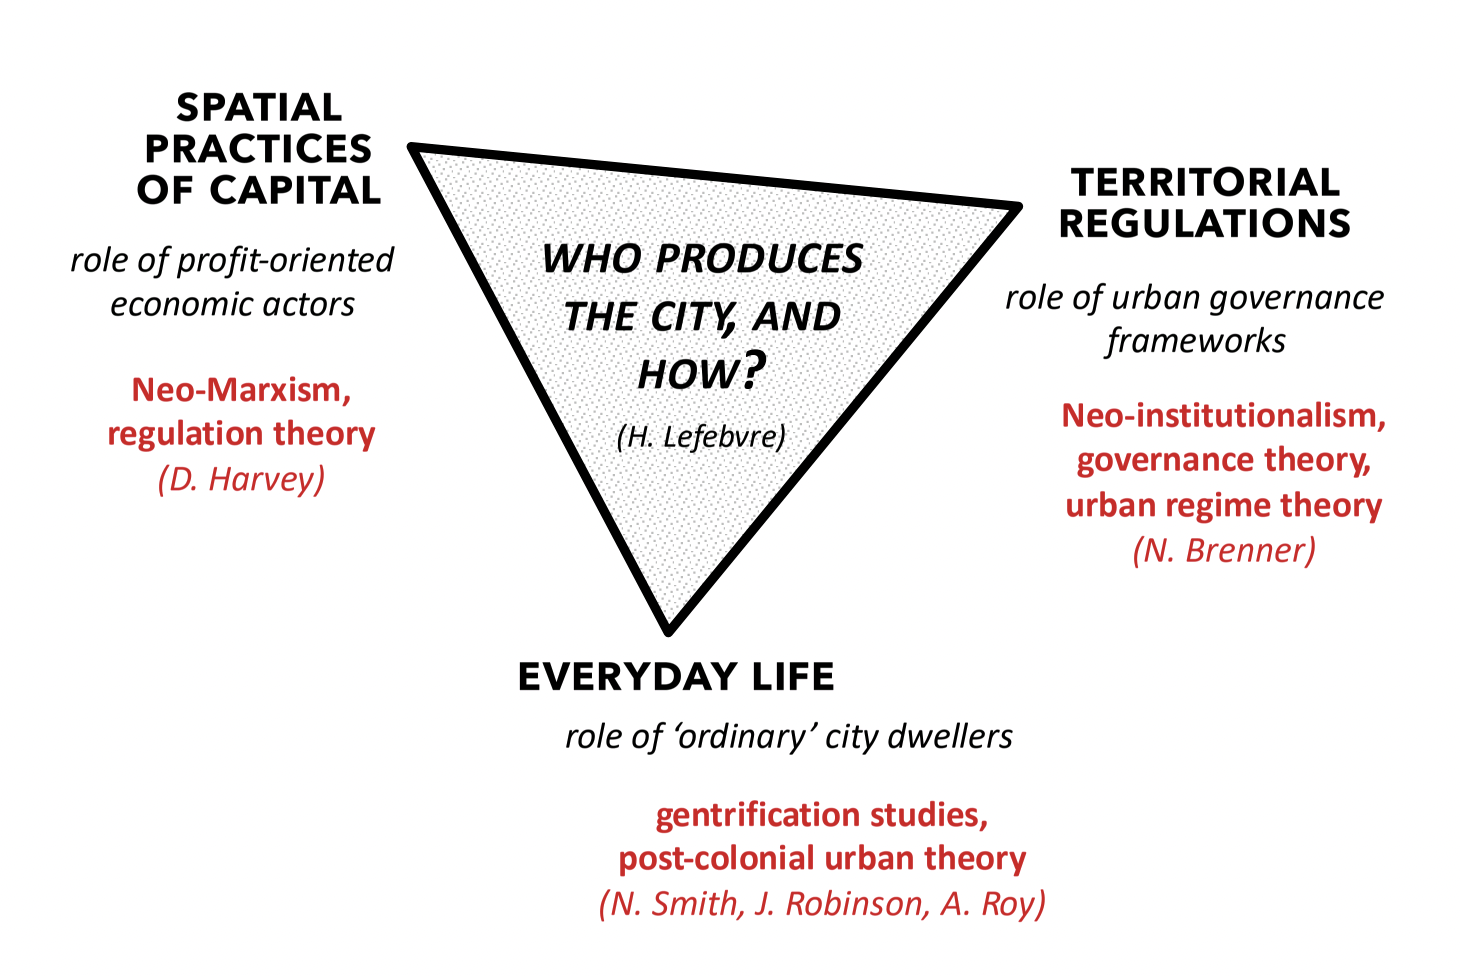
\includegraphics[width=\textwidth]{map_course_organisation1}
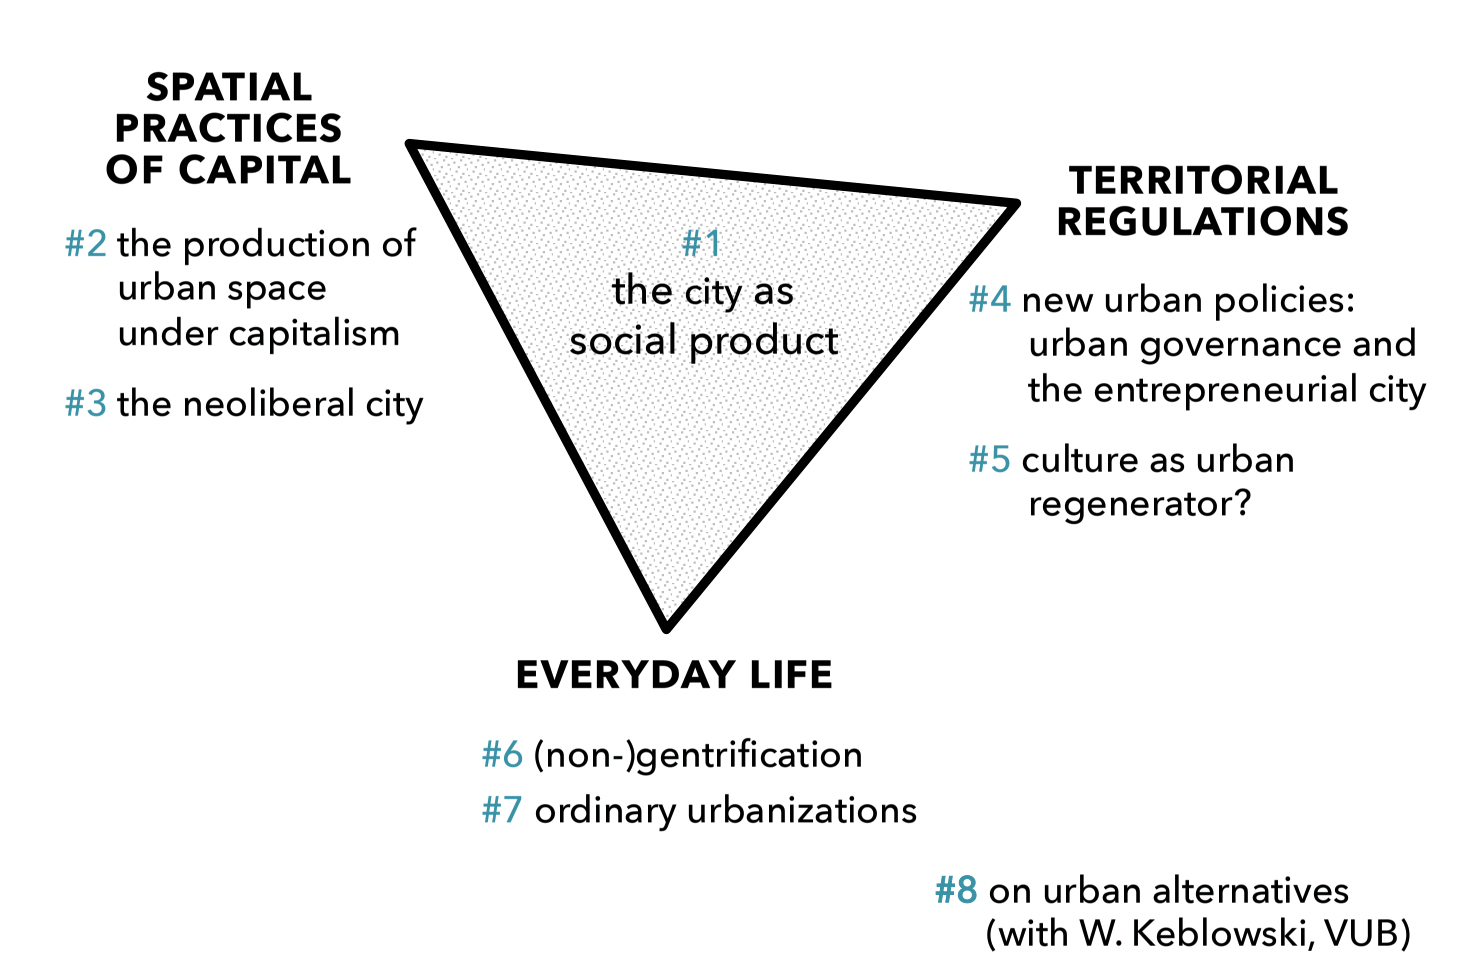
\includegraphics[width=\textwidth]{map_course_organisation2}

%%%%%%%%%%%%%%%%%%%%%%%%%%%%%%%%%%%%%%%%
% 				 LECTURE 2
%%%%%%%%%%%%%%%%%%%%%%%%%%%%%%%%%%%%%%%%

\section{The Production of Urban Space Under Capitalism}
\date{October 7th, 2021}

\textit{tldr; Harvey's theory of the production of urban space under capitalism}

\subsection{Evolution of Urban Space}

What do you think about when you think of urban landscapes? $\rightarrow$ standardisation and copy/past urbanism, shopping streets, high streets; gated communities, suburbanisation, landscapes of dispossession; Dubai, skyscrapers, American malls with extensive parking lots; inequality landscapes; CBD (Central Business District)

We could think of:

\begin{outline}
	\1 Shanghai: from 1990 to 2014, it became a metropolis, China entered the world trade organisation and became a super power
	\1 Panama City: from 1930s to 2010s, became a haven for tax-evasion and offshoring of wealth; came to light with Panama papers
	\1 Cleveland Ohio: in 2008, had many foreclosures due to financial crisis, landscape of abandonment and dispossession 
\end{outline}

\subsubsection{David Harvey}

David Harvey had a theoretical project \textbf{``to integrate an understanding of processes of urbanisation and built environment formation into the general theory of the laws of motion of capital''}, ie. how does urbanisation help us understand capitalism.

He asks the questions:

\begin{outline}
	\1 How and why does capitalism (re)shape (urban) space?
	\1 What's structural about the urbanisation of capitalism, and what's historically/geographically contingent?
	\1 How does the restless character of capitalism (crises, booms, busts...) affect cities?
	\1 How and why does the capitalist production of space bring uneven spatial development?
\end{outline}

\subsection{Capitalism and urbanisation}

\subsubsection{Capitalism}

Capitalism is a system of economic production based on the circulation, or exchange, of privately-owned capital and geared towards capital accumulation. 

Under capitalism, you must re-invest your profit, otherwise other actors will out-compete you (and put you out of business). You also want public or private investors to invest in your business, and such financial investments have grown so much as to become problematic\footnote{The financial investment space is not something I understand well; general understanding is that banks, or finance institutions, lend money/invest, ie. give credit, which means the businesses/people must pay back this money plus interest, and this means they must make a profit. And this has become a problem, because loans cannot be paid back correctly or on time?} 

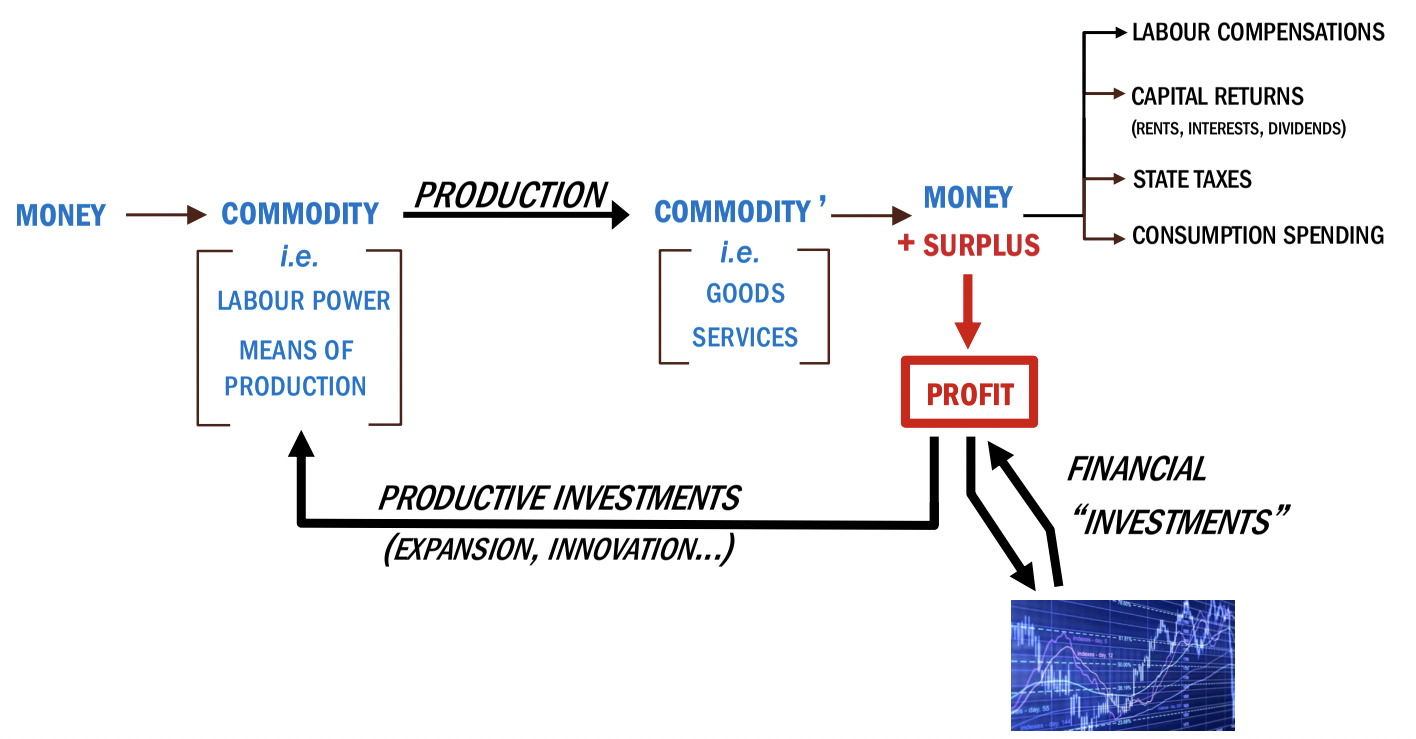
\includegraphics[width=\textwidth]{capitalism}

Thus, capitalism:
\begin{outline}
	\1 An ever-expanding system: capitalism must grow
	\1 Has a geography: it isn't the same everywhere, it's embedded in varying social, cultural, institutional configurations (eg. colonial capitalism, war capitalism, State-controlled capitalism...)
	\1 Has a history: it evolved over time, from a merchant capitalism (16-17th century) $\rightarrow$ liberal industrial capitalism (18-19th century) $\rightarrow$ Fordist/Keynesian industrial capitalism (20th century) $\rightarrow$ neoliberal capitalism (late 20th century)
\end{outline}

%\subsubsection{Capitalism and urbanisation} 

Can we say that cities are created by capitalism? No, cities are not creations of capitalism and existed prior to it. However, the rise and extension of capitalism is deeply linked to the urbanisation process: the emergence of merchant capitalism in Europe's medieval cities, and the massive urban transition since the rise of industrial capitalism, are two eras where capitalism sped up urbanisation.

\subsubsection{A crisis-prone system}

Capitalism is crisis prone, but it has been resilient through history\footnote{China's Evergrande crisis: the collapse of China's second biggest property developer created fear that China's financial system could collapse, however, it did not.}. 

\begin{outline}
	\1 Accumulation is at risk when surplus capital has no outlet in sight for profitable reinvestment, because the circulation of capital cannot continue
	\1 If an outlet is not found, the financial bubble crashes, there are plant closures, social upheavals, geopolitical conflicts...
\end{outline}


Harvey focuses on capitalism's crises. His guiding question is, throughout history, how has capitalism emerged from its periodic crises and found ways to expand further?

\subsection{A theory of urbanisation under capitalism - `fix'}

A `fix' can be one of three things: to put something in place; to repair something; to satisfy an addiction. In capitalism, a fix is a \textbf{temporary `solution' to capitalism's inner crisis tendencies.}

\textbf{Technology fix}: reinvestment of surplus of capital in new or improved production capacities, ie. new sectors and products fuelled by technological and organisational innovations $\rightarrow$ new rounds of growth

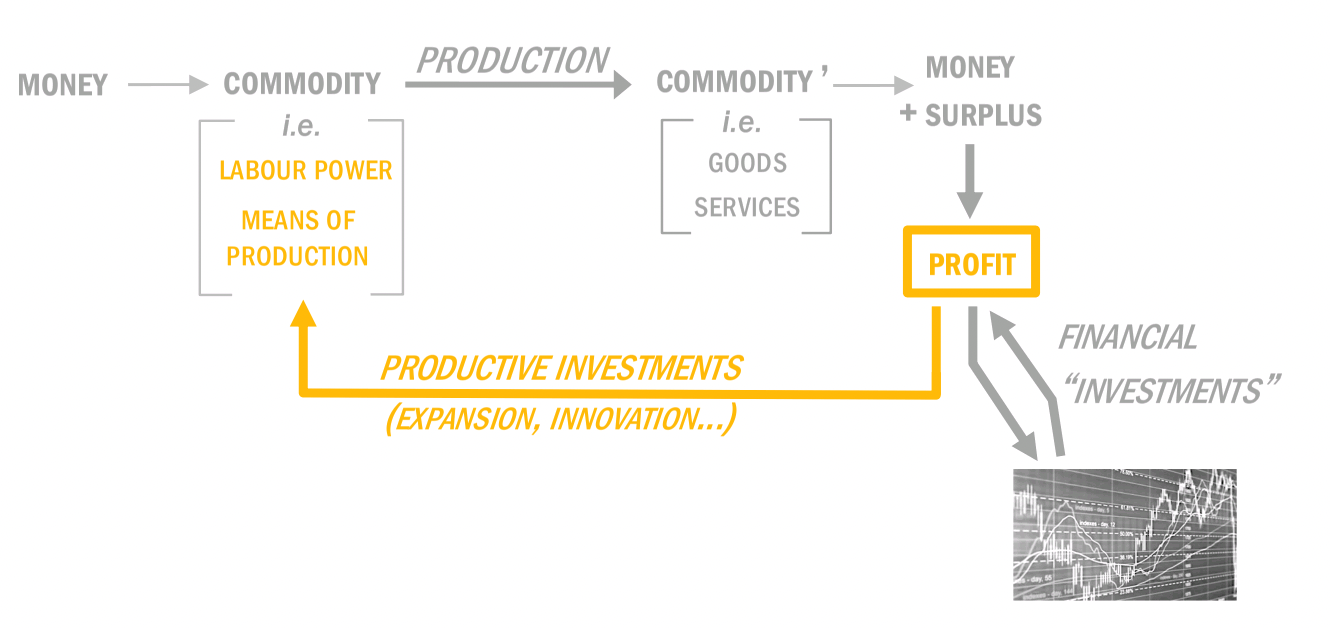
\includegraphics[width=\textwidth]{technological_fix}

\textbf{Financial fix}: reinvestment of surplus capital into financial assets (shares, securities, debt claims...) for the sake of rents and capital gains. This is `financialisation' of capitalism\footnote{For financialisation of capitalism, refer to class no. 3}

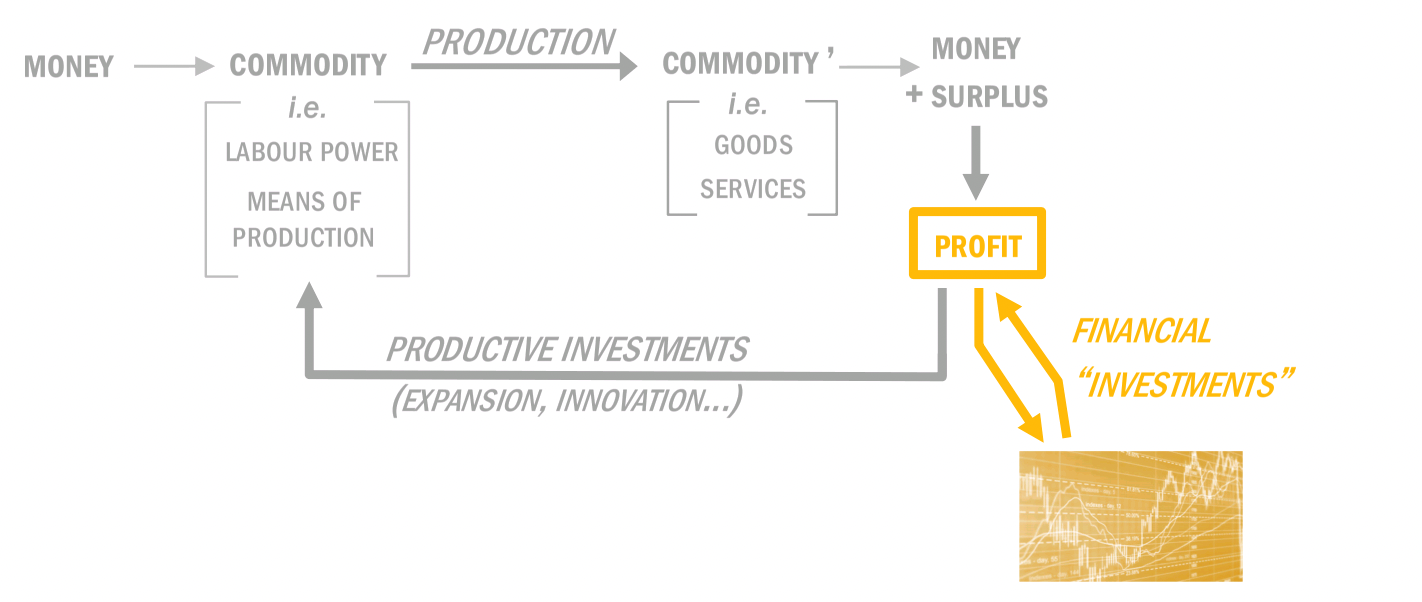
\includegraphics[width=\textwidth]{financial_fix}

\textbf{Spatial fix}: injecting surplus capital into the production of profitable investments. We can observe that the peaks of the construction of tall buildings are not randomly distributed, and are higher at times of crisis (1930s, early 70s, late 80s-90s during the dot com crash and its over optimism, 2008 subprime mortgage crisis).

China and the UAE have the highest number of skyscrapers, and at the same time are places where massive capital surplus exists (or existed at time of building).

\subsubsection{A theory of urbanisation under capitalism}

\begin{enumerate}
	\item Volumes of capital are invested in a selection of localised built environments, in sync with macro-economic temporalities
	\item There is a paradox: investment volumes in the built environment peak in crisis time
\end{enumerate}

Harvey's point is that under capitalism, urbanisation is essential to over capitalism's inner contradictions. \textbf{The production of space is a key outlet for surplus capital and profitable reinvestment} (= spatial fix). ``Capitalism ... is addicted to geographical expansion much as it is addicted to technological change and endless expansion through economic growth''.

The addiction the geographical expansion is both horizontal (taking up more surface area), and vertical (buildings are as high as possible to take in the highest number of people or businesses).

Capitalism is after new spaces of industrial production, of transport and logistics, of consumption, of rent speculation, and new urban markets (eg. airbnb\footnote{In Brussels, Airbnb represents $<$1\% of the housing market, relatively small but Brussels isn't the biggest tourist destination; it is unequally distributed throughout the city, and is concentrated in the city centre, the EU quarter, and the train stations; Airbnb created a new market, which was originally a sharing economy (sharing a room when you are away)}).

\textit{Will this theory still apply when almost all of the world is urbanised?} Yes, because there is creative destruction of urban space. NYC was completely urbanised int he 80s, yet continues to grow through creative destruction. 

\textit{What is a profitable development?} A development that absorbs capital surplus and surplus labour force. It will bring capital back to the investors, who invest speculatively. For the sake of `fixing' capitalism, the fix is consumed as soon as the capital is spent in the development, even before the development is completed and profit has come. 

\subsubsection{Any fix is short-lived}

Under capitalism, any fix is short-lived, temporary. 

\begin{outline}
	\1 Paris' Haussmannisation, 1853-1868: Paris was in a time of severe crisis, with the revolution in 1838. Napoleon III arrives rises to power in 1852 and appoints Haussmann to develop the city. 
		\2 Haussmann develops profitable outlets like the Grands Magasins, the Opera
		\2 There is a massive transformation from the medieval character of Paris (tiny, dirty streets) to grand, clean avenues
		\2 This type of development requires a massive amount of capital
		\2 In \textit{The Housing Question}, 1872, Engels questions the legitimacy of Haussmann: the plan was to make Paris more liveable, but did it consider the people who were currently living there? Will they be back in the new buildings that replaced the `slums' and `ghettos'?
	\1 Post-war capitalism and urbanisation (jobless demonstration in Chicago, in 1934)
		\2 Technology fix: investment in mass production of durable consumer goods by industries organised along Fordist principles, to be consumed by expanding national customer markets supported by Keynesian economics
		\2 Financial fix: massive allocation of capital into the credit system, towards companies, households (mortgage credits, consumption credits) and State authorities (debt-financed public works and infrastructure, eg. New Deal, Marshall Plan)
		\2 Spatial fix: massive investment in urban expansion (housing, infrastructure, highways) fuelling a huge wave of suburban growth centred on middle-class habitat and consumption patterns
\end{outline}

\subsection{Suburbanisation}

Picture LA, with miles and miles of single family housing; the American dream of owning a private house with a backyard and a car, almost regardless of the commute and community (or lack thereof);

See \textit{Suburban Planet}, Roger Keil.

Suburbanisation is not a middle-class phenomenon. Low income households are now moving away from dense urban centres, especially when inner-city neighbourhoods become gentrified and expensive.

\subsubsection{The case of Belgium}

Belgium's policies favoured the development of housing along the motorways that connect cities together, and it is a particularity of Belgium to have a lot of motorways (0,2km of motorway per person in Belgium, twice as much as in France). The intense development of the motorways created a favourable environment for Belgians to built their own house, and the ideal became to have a house `far away' from another, with a (company) car (preferably a company car). 

There is a saying that ``Belgians have a brick in their stomach'', meaning that they are born wanting to build a house.

\subsection{Summary the theory of urbanisation under capitalism}

\begin{outline}
	\1 Capitalism has an \textbf{insatiable addiction to the production} of (profitable) space, for this is a key way to overcome its own contradictions
	\1Under capitalism, \textbf{the mobilisation of urban change for the sake of capital accumulation is permanent}, but lays at the forefront in crisis times
	\1 Under capitalism, \textbf{any spatial fix is short-lived}, for the (profitable) way out of a crisis paves the way to the next crisis
	\1 Under capitalism, \textbf{fixing space has ramifications}, on the built environment but also on modes on consumption, mobility patterns, cultural and political subjectivities
	\1 \textbf{Under capitalism, any spatial fix comes with patterns of uneven spatial development}
\end{outline}

\subsection{Uneven spatial development}

Under capitalism, patterns of investment in some places are structurally associated with patterns of \textbf{disinvestment} elsewhere. Creative destruction displaces communities who are not allowed to return afterwards.

\begin{outline} 
	\1 t0: selected places are dynamic edges of capitalist urbanisation, for their production participates in a spatial fix
	\1 t0 $\rightarrow$ t1: progressively, those places lose their fit vis-a-vis evolving capital requirements
	\1 t1: capital fixed in the those places is devaluated, for new places are now more profitable for investment, or they become local barriers to new rounds of accumulation
	\1 t1 $\rightarrow$ t2: capital moves elsewhere, or is invested in a `creative destruction' of local space
	\1 t2: capital moves back in restructured places, that appear attractive once again under new circumstances
\end{outline}

There is a cyclic dimension to the spatial fix: capitalism doesn't solve crisis, but moves them around geographically. 

Take the examples of Ny-Lon-Kong (NY, London, Hong Kong) and Detroit. These two places are part of the same story. The investment in one causes the disinvestment in another.

\url{https://www.youtube.com/watch?v=qOP2V_np2c0&ab_channel=RSA}

\subsection{Keywords}

David Harvey
Capitalism
Capitalism's crisis
Production of space
Fix: technological, financial, spatial
Keynesian economics
Creative destruction

%%%%%%%%%%%%%%%%%%%%%%%%%%%%%%%%%%%%%%%%
% 				 LECTURE 3
%%%%%%%%%%%%%%%%%%%%%%%%%%%%%%%%%%%%%%%%

\section{The Neoliberal City}

\textit{tdlr; zooming in to the present conjuncture of the production of space under capitalism, ie. urbanisation under neoliberal capitalism, or the `neoliberal' city. Urban spaces are sites and vehicles for neoliberalism: sites because that is where the accumulation takes places, and vehicles because of the financialisation of the real estate market, and it's speculation. The 21st century city is a city of rents.}

\textbf{Why is housing so expensive in cities?} 

\begin{outline}
	\1 There is a problem of \textbf{supply and demand}: prices are pushed up when the demand is high and the supply low (economic argument). The logical solution would be to boost supply, but interest rates are too low and so people are not selling their properties.
	\1 According to neoliberalists, there is \textbf{too much regulation}, and investors cannot supply enough properties. Exclusionary zoning prevents multi-family housing, there are height restrictions, parking requirements drive prices of housing upwards (for 100 housing units, you need 200 parking spots, which is not possible to find space for anyway). 
	\1 Conservative residents, \textbf{NIMBYs}, participate in community meetings regarding housing developments, and protest against changes
\end{outline}

But, focusing only on supply and demand is limiting. For example in Berlin, the demand is low but the prices are rising. In London, the prices are rising but real estate is also increasing.\footnote{What happens in places where space is not an issue, for example, in Astana?}\marginpar{Astana has `unlimited' space - how does that affect housing market?} 
Renting is a \textbf{``second hand market''}.

\href{https://www.vox.com/22629826/gentrification-definition-housing-racism-segregation-cities}{Vox:  What we talk about when we talk about gentrification}

\subsection{What is neoliberalism?}

Neoliberalism is ``the set of intellectual proposals and political orientations that aim to extend market mechanisms and ethics of competition to an every-wider spectrum of social activities, based on strong state intervention'' (Pinson, 2020)\marginpar{Neoliberalism is the extending of markets, based on state intervention}

Neoliberalism isn't about the privatisation of everything, it isn't `laissez-faire'. 

\begin{outline}
	\1 Neomarxism: neoliberalism is a \textbf{class project to remove restrictions in the way of accumulation} (Harvey)
	\1 Bourdieusian: a State project, with state interventions (Wacquant)
	\1 Foucaldian: a new ethos, or government rationality (Brown)
\end{outline}

\subsection{What's new about neoliberal capitalism}

\subsubsection{20th century trend of capital in the Global North}

From the 1980s, there is a turn from the Fordist-Keynesian era to the \textbf{`post-Fordist', `informational', `flexible', `globalised',... `neoliberal' era}. 

Pre 1980s, the profit rate decreased, and there was a capitalism crisis. Then, things took a \textbf{neoliberal turn}:

From the early 1980s, the profit increased, but the reinvestment rate was low. There is still a growing gap between the \textbf{profit rate} (the return on productive capacities) and the \textbf{accumulation rate} (the share of profit reinvested in productive capacities). Capital has grown, but has not been accumulated (reinvested).

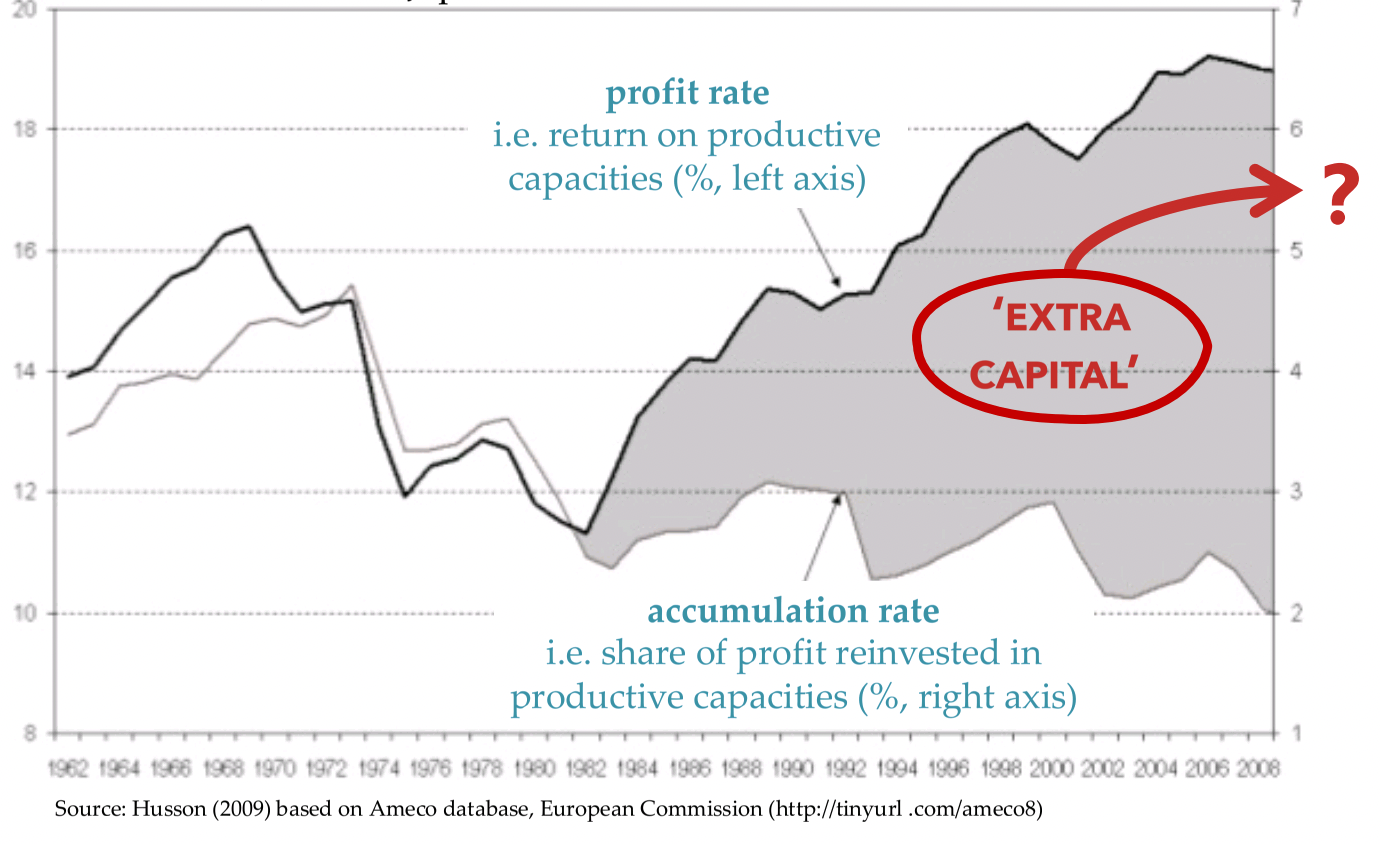
\includegraphics[width=\textwidth]{neoliberal_turn}

The question is, \textbf{what happened to this surplus of capital?} 
It was not reinvested in wages, and taxes did not increase. 

\subsubsection{The surplus of capital}

There was a \textbf{trans-nationalisation}, where capital was invested externally: companies globalised, off-shored and outsourced their production, there were mergers and acquisitions, foreign direct investment

There was also a switch to \textbf{financialisation} of capital, where the surplus went into financial markets

\subsubsection{Transnationalisation}

An increase in Foreign Direct Investment (FDI), ie.  investors establishing long lasting interests in an enterprise residing in another country. 

\subsubsection{Financialisation}

The Dow Jones is a collection of traded companies, ie. companies available through the financial market. Since the 1980s, its value has grown enormously, showing how enormous financialisation has become.

Financialisation:

\begin{outline}
	\1 Is an increasing concentration of capital in the financier's hands
	\1 Uses \textbf{asset valuation} strategies, where the purpose is to valorise a set of assets (what ever an asset can be) and speculate, and thus maximise rental\footnote{Rent is the payment charged by the owner of a property, to a user, in return for its use} yields (dividends, rental income, interest returns...) or capital gains on resale
\end{outline}

Comparing GDP of countries with the largest asset managers, if Germany was an asset manager, that is if all of the German companies (Mercedes, Audi, BMW, etc.) formed an asset management company, they would the 3rd biggest in the world. This shows how huge the concentration of wealth is in financial circles. 

\subsection{In what sense is neoliberalism urban?}

Cities and urban spaces are \textbf{strategic and critical} for neoliberalism:

\begin{outline}
	\1 as critical \textbf{sites} of capital accumulation
	\1 as critical \textbf{vehicles} for capital accumulation
\end{outline}

\subsubsection{Critical sites of accumulation}

\begin{outline}
	\1 \textbf{Global cities}\marginpar{S. Sassen} need to control ever more of the world networks and flows
		\2 There is a \textbf{spatial concentration of strategic command and control functions}
		\2 They are nodes in a global space of flows (money, information, goods, services, workers...). Being an entity in one global city, brings you closer to peers in other global cities, rather than bringing you closer to peers who are geographically closer, but who's city is not global $\rightarrow$ a network of people between global cities, that excludes others from participating if they do not have the same `power'
		\2 Global cities are biased to the Global North
	\1 \textbf{Worlding cities} (A. Roy, A. Ong) are cities emerging as global cities
		\2 Typically from the Global South, and from emerging countries (Shanghai, Singapore, Hong Kong, Taipei, Mumbai, Doha, Dubai, Rio de Janeiro, Johannesburg...)
	\1 \textbf{Globalisation from below} (A. Portès) 
		\2 Places of production and consumption associated with transnational communities sitting astride political borders
		\2 For example, Marseille, or Rue Heyvaert in Brussels where European cars are shipped to North Africa and the Middle East
	\1 \textbf{Inconspicuous cities beyond global cities} (A. Choplin, O. Pliez)
		\2 Secondary cities should be given more consideration
		\2 Global cities invest in such cities, and thus they are crucial for how capital accumulation works
	\1 \textbf{Urban peripheries}
		\2 Global suburbanism (R. Keil)
		\2 Planetary urbanisation (Brenner and Schmidt) is about the implosions and explosions, the concentration and the extension of urbanism. Planetary urbanisation means that spaces that are far away from the city cores and suburban peripheries, are strongly linked to urbanism and urbanisation. For example, Alberta, Canada's oil fields are fuelling an urban lifestyle
\end{outline}

\subsubsection{Critical vehicles of accumulation}

The Battersea Power Station in London sold for 1.6bn gbp to a Malaysian fund. The power state is a landscape of cranes, building housing units/leisure/business spaces, but it isn't a local project.

\begin{outline}
	\1 There is a growing \textbf{financialisation} of urban development
		\2 Huge amount of capital goes into commercial real estate markets (retail, office, housing, logistics) since the late 1990s
			\3 Capital switched around the 2000 dot com crash, from internet companies to real estate (leading to the subprime mortgage loans)
			\3 This led to the subprime mortgage crisis, and we see that one crisis creates another
			\3 Highly uneven geography, where Global North and global cities have significant investments, and \textbf{capital converges} 
		\2 Increased coupling of real estate activity to market finance
			\3 Rise of real estate asset management
			\3 Strategies of \textbf{assetisation}, to turn real estate (land, property) into financial assets to be treated as such
	\1 From assetisation of real estate to \textbf{speculative urbanisation}
		\2 The mobilisation of land or property for the sake of maximising rent extraction.
		\2 Speculation is trying to extract as much money from your property. Land is mobalised
		\2 The 21st century metropolis is a \textbf{city of rent}\marginpar{Samual Stein, \textit{Capital City}}
\end{outline}

\subsection{The 21st century city of rent}

There are multiple expressions:

\begin{outline}
	\1 The rise of corporate landlords and buy-to-let housing markets
	\1 Speculative projects tailored to meet investor's requirements first
	\1 Increased tendency of urban governments to rely on the real estate valorisation of their land resources in order to finance public utilities
	\1 Growing un-affordability as a systemic feature, because profit is necessary
		\2 Highlights the uneven geography, as investments rise in one place (= city growth) and leaves other places behind (= shrinking cities).
\end{outline}

\textit{\textbf{$\Rightarrow$ Neoliberal urbanisation as “neo-Haussmannization” (Merrifield, 2014), “generalized gentrification” (Smith, 2002), “planetary gentrification” (Lees, Shin, Lopez-Morales, 2016), a regime of “expulsions” (Sassen, 2014), “accumulation by dispossession” (Harvey, 2003)}}

%%%%%%%%%%%%%%%%%%%%%%%%%%%%%%%%%%%%%%%%
% 				 LECTURE 4
%%%%%%%%%%%%%%%%%%%%%%%%%%%%%%%%%%%%%%%%

\section{New Urban Policies: Urban Governance and the Entrepreneurial City}

\textit{tldr; capitalism isn't the only force shaping the city. Urban governance and the entrepreneurial city play an increasing role in shaping urban space}

To think capital  alone shapes cities is too simplistic, not only economic structure; depart from purely structuralist approach;

markets are politically organised, made possible through institutional arrangements 
	- how to make sense of mediation by institutional arrangements?
	- among the institutional arrangements, the state institutions are undeniably key players 

\textbf{How to make sense of the role of the State in contemporary urban changes?}

-Neo-institutionalism
	- consider much broader range of public actors, and those interacting with state institutions (ngos, lobbies....) 

- Neoliberalisation of urbanism

in contrast to the urbanisation of neoliberalism (from previous lecture)

\subsection{Creative destruction of the state}

In contrast to the creative destruction of economic structures (previous lecture)

\textbf{What's new with recent urban politics?}

\subsection{Rescaling of statehood}

Brenner\footnote{Neil Brenner, \textit{New State Spaces}} follows Harvey's theory, that capital cannot find outlet and thus finds the urban. 
Core argument: re-configuration of economic structures (1980s), and re-organisation of state regulation -> rescaling of Statehood, to make difference between state as an institution, and statehood which is abstract idea. Statehood = public power, public authorities, all the forms through which public power is exercised. Detach from specific scale

Emergence of less national-centric form of Statehood - national states have not been eliminated, but this rescaling of the scale of public regulation (eg. of capital flows), has brought more importance to other scale than national one.

- upscaling: supra national tiers of government (EU)
- downscaling: devolution towards subnational tiers (Belgium regions, Netherlands provinces, German landers)
- outsourcing: towards private and civiil society actors

All together, the complete picture is an increased relevance of urban/regional scale of state power (Statehood), regarding production and development of urban policy.
Global architecture of State power is multi-layered, and the urban scale has a greater importance than before.

New transnational network of city governments (like euro cities, c40 cities mayors summit, resilient city networks,... ). Usually such transnational organisations are on the nation level, not city.

The point of rescaling statehood is not like Glaeser on the triumph of the city, where governments are not able to face challenges of 21st century
Instead, Brenner says we are in a multi-layered, less national centric form of Statehood 

In the background: less national to local transfers for investment capacities.
Eg. vision of North Quarter in Brussels in the 1960s, to be transformed as a global financial centre (mimicking NYC with the world trade centres). Development of world trade towers was complete failure, and the consequences are still seen: Northern Quarter is not a great livable place.

At that time, such developments were made at the national level. These would not take place anymore, the scale of ``who decides'' is completely different, and the role of regional authorities is central now -> rise of urban governance

\subsection{Rise of urban governance}

Why governance instead of government -> a diversification and widening of stakeholders involved in the urban policy making

Urban governance reoriented the debate on political power in cities, beyond Government and Parliament, towards a production of the ``capacity to govern''.
People who have the material and symbolic capacity to govern, may not be the ones in the seats of government

\textbf{Urban regime theory}: assumes that no one in the city holds all the resources and capital necessary to have enough impact to produce urban policy, and urban projects. The capacity to produce is distributed amongst many hands.
Urban politics is the activity to assemble these resources (stakeholders, institutions) together, and find a consensus, in order to have the capacity for a stable amount of time (years). The urban regime is an informal coalition, of stakeholders bringing different resources (money, legislative power, symbolic power). There is no `office' of the urban regime
The stakeholders all have the common interest of growing the economy.

Example of Tour et Taxis:
- An industrial site, warehousing, freights, with large rail station for goods, not people
- Emptied in the 80s, redeveloped since then
- A historic site, supposed to be a multifunctional neighbourhood with housing, offices, leisure, event spaces, green space... the largest development in Brussels
- Who is developing this? Share holding company bought it from port authority; use money from bank institutions and investors; using this money, they bring in construction companies; they have two important tenants (administrations), events are taking place (attract people, the media, radio); site is in the Brussels region, but regional government is also involved; etc., a MULTI-stakeholder project

Through what channels does this ``assemblage'' become effective?
- public-private partnerships (PPP): eg Villo partnership between brussels region and JCDecaux
- citizens' participation frameworks
- strategic planning

\subsubsection{Public private partnership (PPP)}
- a legally binding contract between a private actor and public authority for development of a facility
- Private company often have DBFM-O contracts: design, build, finance, maintain and operate \marginpar{Are Astana buildings PPP?}
- Public authority: contributes by land allocations, tax cuts...
- Users pay a fee for the facility, such that after some years the facility will be owned by the state

Eg. Øresund bridge between Malmö and Copenhaguen

Pros:
- It limits indebtedness, because the public authority doesn't have to borrow money in the first place
- The public authority doesn't have to fund the civil servants to run the facility, because the PPP will take care of it

Cons:
- In the long run, its more costly for public finance: you have to pay the contractor, plus their profit, because the private contractor seeks a return on investment
- Not hiring civil servants is a loss of expertise; no one in the public administration knows how to manage the infrastructures/equipments
- Empowers private actors to direct the allocation of public funds
- Raises issues about democratic control, because only the parliament will have visibility over the spending. PPP contracts are not public documents

Some governments have decided to not have PPPs for eg. hospitals - after 30 years when the government owns the site, you don't have control over the state of the site

\subsubsection{Citizen participation framework}

``Participatory turn'' in urban politics: platforms, councils...

The rationale is to bring policy-making to be more `open' and `responsive' to citizens

Recurrent limitations and biases:
- Categories of populations participate more than others: ethnic, demographic, owner/renter biases
- Equalising levels of information: there are time tensions, because elected people running the participatory turns, want it to be a fast process. However, the experts' speed is much too quick for the participating inhabitants
- `Local trap': looking at the scale of neighbourhood/site, keeps the wider picture out of sight and discussion. As if all local problems can be solved locally, but sometimes they have to involve wider picture.

S. Arnstein's \textit{A Ladder of Citizen Participation} asks, how much power is actually transferred to citizens in the participatory frameworks?

\subsubsection{Strategic urban planning}

A strategic, or project based, turn in urban planning. 

Land use map: 100\% of territory is zoned, a zone defines regulations about the place (what is allowed, or not)

Strategic plans: clearly not a land use plan, less detailed, and some zones are not highlighted. It shows priorities and strategic options for the city's future development, including lines that cross the regional boundary
- a consensus building tool, a way to mobilise diverse stakeholders around how the city should be developed in spatial terms; a project based orientation

\subsection{Rise of urban entrepreneurialism}

\url{www.worldbank.org/competitivecities}

What is the entrepreneurial script?
- Views the city as a company, in a market environment, which must be competitive
- A successful city means growth
- Make the city look like a business friendly environment: relax regulation/lower taxes, improve infrastructure, provide incentives, boost city's image...
- Many blind sports: shared prosperity for all? how so? is this automatic? -> Being competitive means that some cities are winning, and some are losing. Urban development is not equal. \marginpar{ASTANA! Not shared prosperity for all, even within the city}
- One recipe does not fit all, there are diversity of local contexts... cities should not all run the same race. Cities should not all be doing the same thing
- Governments should make the city a friendly and attractive place for environments, but should not focus on a single type of business; what about other parts of the economy that make a city, like schools, theatres, hospitals etc. (ULB doesn't have to be attracted to Brussels).
Cities aren't only 'entrepreneurial', and do much more, but competition is usually considered the path to success

Entrepreneurial city:
- mainstream in urban/regional policy
- often kept outside the space of debate, "TINA" there is no alternative, it's a post-colonial condition (Swyngedouw)
- focuses on 3 dimensions:

\subsubsection{Inter-urban competition}
	- inter-urban competition: cognitive matrix; `competition', `entrepreneurialism' as critical concepts; way to take a critical look at evolution of urban governance; you need to be competitive, otherwise you will decline; 
	this is not intuitive - how can you imagine that Brussels is in competition with anyone in Amsterdam? residents, hairdressers, hospitals, don't feel in competition with those in Amsterdam; 
	So, where does it come from? 
		- model of new public management, to make public administration more business-like to improve efficiency of public services; use competitive forms of resource allocation (eg. project based funding); -> creative destruction of the state
		- Increased trans/intra national mobility of capital -> creative destruction of the economy
	- An example of inter-urban comptetition: Amazon HQ2, asked for cities to bid to have their 2nd headquarter, promising to create 50k jobs (HQ1 in Seattle); they had many requests (tax breaks, geographical preferences); several hundred cities bid;
		- Inter-urban competition is not natural, cities aren't in competition, but are put in competition with each other by powerful actors (like amazon)
		- Intensity of inter-urban competition is historical and geographical; depends on existing regulatory frameworks
	
\subsubsection{Supply side economics as development  strategy}

	- supply side economics as a development strategy
		- invest in the quality of the place -> urban competitiveness-> economic growth -> trickle down effects (activity, jobs, tax returns...) ->.invest in quality of place x

``trickle down economics have never worked'' --> instead of betting for amazon, fund the city itself. don't wait for amazon to come in and fix the network. you have to grow the city from the bottom and middle out, not at the top

\subsubsection{Symbolic policies}

- \textbf{City marketing} - promoting local advantages of a place, this is not a new concept
- \textbf{City branding} is new; all cities now have a logo, but the logo does not say much or anything about the city, it just helps to build a brand, just like companies; advertising techniques applied to cities, and producing a desire, speaking to the heart and feelings, and not to the head, of potential customers; building attachment to a place;
	- eg. I love NY; \marginpar{Is there an astana city brand?}


%%%%%%%%%%%%%%%%%%%%%%%%%%%%%%%%%%%%%%%%
%				 LECTURE 5
%%%%%%%%%%%%%%%%%%%%%%%%%%%%%%%%%%%%%%%%

\section{Culture as Urban Regenerator?}

%%%%%%%%%%%%%%%%%%%%%%%%%%%%%%%%%%%%%%%%
%				 LECTURE 6
%%%%%%%%%%%%%%%%%%%%%%%%%%%%%%%%%%%%%%%%

\section{(Non-) Gentrification}

%%%%%%%%%%%%%%%%%%%%%%%%%%%%%%%%%%%%%%%% 
%				 LECTURE 7
%%%%%%%%%%%%%%%%%%%%%%%%%%%%%%%%%%%%%%%%

\section{Ordinary Urbanizations}

%%%%%%%%%%%%%%%%%%%%%%%%%%%%%%%%%%%%%%%% 
%				LECTURE 8
%%%%%%%%%%%%%%%%%%%%%%%%%%%%%%%%%%%%%%%%

\section{On Urban Alternatives}

%%%%%%%%%%%%%%%%%%%%%%%%%%%%%%%%%%%%%%%% 
%				READINGS
%%%%%%%%%%%%%%%%%%%%%%%%%%%%%%%%%%%%%%%%

\section{Readings}

\subsection{The Neoliberal City}

\subsubsection{Charmes, Rousseau, \textit{Planetary Globalisation}}

\begin{outline}
	\1 The covid 19 pandemic could serve as empirical evidence to \textbf{planetary globalisation}, in support of Brenner and Schmidt's new theories and hypothesis that we need completely new methods of analysing urbanisation
	\1 Planetary urbanisation is intrinsically linked to the globalisation of capitalism via these processes: disappearance of ``wild'' zones, global interconnectedness of territories, blurred division between town and country, and globalisation of urban inequalities
	\1 ``Wild zones'': places where (wild) animal diseases that humans contract come from; zoonotic diseases represent 60\% of human diseases. The fact that we contract them, mostly from livestock interacting with wild animals, is a sign of the scale of urbanisation: there are no ``wild'' places anymore. Urbanisation is taking over wilderness, upsetting ecosystems, creating new contacts between humans, plants and animals.
		\2 Places where urbanisation is most intense are places where infectious diseases start (China, West Africa, Middle East)
	\1 Global interconnectedness of territories: there are massive urban entities and they interact with the entire planet almost simultaneously. 
		\2 Covid 19 was able to spread so quickly because of high traffic around the world; governments were not prepared for such a rapid spread, because urbanisation was ill-understood as planetary. 
		\2 The flows of goods are increasingly complex and multiform: China does not manufacture ready made objects. Flows are \textbf{delocalised} and manufacturing chains are globalised
	\1 Blurred division of town and country: a metropolis can no longer be considered only as a vertical city
		\2 It is a place of interlacing networks, providing daily links with places and people that have various forms, sizes and functions
	\1 Planetarisation of urban inequalities:
		\2 Spatial inequalities was boosted by the first cities, which extracted food surplus from the hinterlands, in order to feed a population that, for the first time, no longer needed to burden themselves with the production of food (that became known as the bourgeoisie). The bourgeoisie started accumulating goods, and space, and this laid the foundation of capitalism
		\2 Gradually, urbanisation took over from industrialisation as the main driver for capitalism The globalisation of capitalism is the main driver of the inequality of territories
		\2  Gentrification is a process of segregation, and can be seen on a global scale: the rich take over space that was previously used/inhabited by low-income, working class, and push these people further out to the fringe of a city.
		\2 There is a link between wealth and the spread of disease: the upper classes travel more, thus are more likely to spread the disease. Contagion is `elitist', and especially so during the covid 19 pandemic because of the price (or the targets) of testing
\end{outline}

\subsubsection{Peck, Theodore, Brenner, \textit{Neoliberal Urbanism: Models, Moments, Mutations}}

\textbf{Neoliberalism}: free market, unrestrained, global capitalism

\begin{outline}
	\1 Path dependence between neoliberal restructuring, and institutional and spatial landscapes
\end{outline}

\subsubsection{Peck, Theodore, Brenner, \textit{Neoliberal Urbanism: Models, Moments, Mutations}}

\subsection{New Urban Policies: Urban Governance and the Entrepreneurial City}

\subsubsection{Pinson, Morel Journel, \textit{The Neoliberal City - Theory, Evidence, Debates}, 2016}

\begin{outline}
	\1 There are different waves of neoliberalist theory:
		\2 Historically, it was economic. Neoliberalism is a fluid movement of ideas
		\2 Bourdieu: neoliberalism is a political movement, a new articulation of state/market/citizenship
		\2 Foucault: new regimes of governmentality with rise of technology, competition. A new rationality
		\2 Neo-marxist: project to restore conditions for capitalist accumulation, a class project
	\1
\end{outline}

%%%%%%%%%%%%%%%%%%%%%%%%%%%%%%%%%%%%%%%% 
%				ENVIRONMENTS
%%%%%%%%%%%%%%%%%%%%%%%%%%%%%%%%%%%%%%%%

\begin{outline}
	\1
\end{outline}


\end{document}